% \clearpage
\secrel{Smart Watch}

\noindent
Personal Planning is the topmost domain where a smartwatch can be used as
control terminal or primary computing device. The Watch is always on and ready
to use in a second: it can notify you about events from planning software,
display actual tasks and near locations using GPS.

And you can push button to make a new task “I want something to add” which will
poll you until you modify\note{using editor on your phone} it to the real task
you want to add.

Also, you can think about your smartwatch as IoT device \ref{iot}\ able to
collect some data for analysis and prediction. Your watch will collect data
continuously, send it to the north side of IoT cloud, and software\note{you can
write it yourself for special tasks, or use third party modules} runs there do
processing and sends back events and notifications for you.

Modern watches have a lot of health sensors, GPS, light and temperature sensors
— it is good data source to make predictions and guessing in personal planning
software: it can use task database\note{what you need to do}, resource
information\note{money and goods you have or will have some time later in a
prediction} and use deep learning to dynamically advise you right into your
current life moment what to do\note{notifications starting from dumb alarms,
time planning, resource/budget accounting,\ldots}.

\noindent
\begin{tabular}{l p{0.75\textwidth}}
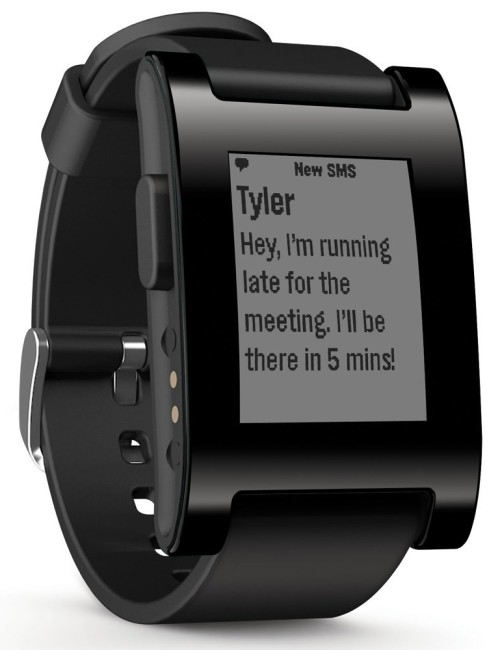
\includegraphics[height=0.45\textheight,valign=t]{img/pebble_classic.png}
&
I have this one Pebble Classic myself. It's an old smartwatch, which has BT
connection with host software on the mobile phone but can work standalone a long
time (more than two weeks without recharge). It is lightweight, adjustable and
can be good terminal for instant planning.
\\
\end{tabular}
This device was done on a light SMT32 microcontroller, and you can program it in
pure C using online Pebble SDK. It was not treated as one of targets for \uF, as
it has no keyboard or remote terminal. Here I
\href{https://www.quora.com/unanswered/How-can-I-write-remote-terminal-Android-for-Pebble-Classic-Smartwatch-to-be-able-to-reprogram-it-interactively-I-think-about-full-watch-hosted-Forth-port-or-tiny-bytecode-interpreter-and-compiler-embedded-into-the}{asked
about terminal} able to work on mobile phone, and let to interact with Pebble in
a live session. Still have no working decision.

\bigskip
More modern SmartWatches available now uses Google's
\href{https://www.android.com/wear/}{Android Wear}. It makes them annoying in
everyday recharging, but this platform and hardware have more power to be able
to work standalone as primary planning computing platform.
